%%%%%%%%%%%%%%%%%%%%%%%%%%%%%%%%%%%%%%%%%
% Simple Sectioned Essay Template
% LaTeX Template
%
% This template has been downloaded from:
% http://www.latextemplates.com
%
% Note:
% The \lipsum[#] commands throughout this template generate dummy text
% to fill the template out. These commands should all be removed when
% writing essay content.
%
%%%%%%%%%%%%%%%%%%%%%%%%%%%%%%%%%%%%%%%%%

%----------------------------------------------------------------------------------------
%	PACKAGES AND OTHER DOCUMENT CONFIGURATIONS
%----------------------------------------------------------------------------------------

\documentclass[12pt]{article} % Default font size is 12pt, it can be changed here

\usepackage{natbib}
\bibliographystyle{plainnat}
\usepackage{url}

\usepackage{soul}

% latex configuration
\usepackage{listings}
\renewcommand*{\lstlistingname}{Code} % replace the label
\lstset{
	belowcaptionskip=1\baselineskip,
	frame=L,
	xleftmargin=\parindent,
	showstringspaces=false,
	basicstyle=\footnotesize\ttfamily %font family
}

\usepackage[portuges]{babel}
\usepackage[utf8]{inputenc} % Acentuação
\usepackage{indentfirst}
%\setlength{\parskip}{\baselineskip} % Space between paragraphs
\usepackage{parskip}% http://ctan.org/pkg/parskip

\usepackage{geometry} % Required to change the page size to A4
\geometry{a4paper} % Set the page size to be A4 as opposed to the default US Letter
% For right aligend descriptions
\usepackage{calc}
\usepackage{enumitem}

\usepackage{graphicx} % Required for including pictures

\usepackage{float} % Allows putting an [H] in \begin{figure} to specify the exact location of the figure
\usepackage{wrapfig} % Allows in-line images such as the example fish picture

\usepackage{lipsum} % Used for inserting dummy 'Lorem ipsum' text into the template

\linespread{1.2} % Line spacing

%\setlength\parindent{0pt} % Uncomment to remove all indentation from paragraphs

\graphicspath{{./pictures/}} % Specifies the directory where pictures are stored

\begin{document}

%---------------------------------------------------------------------------------------
%	TITLE PAGE
%---------------------------------------------------------------------------------------

\begin{titlepage}

  \newcommand{\HRule}{\rule{\linewidth}{0.5mm}} % Defines a new command for the horizontal lines, change thickness here

  \center % Center everything on the page

  \includegraphics{logo}\\[1cm] % Include a department/university logo - this will require the graphicx package

  \textsc{\LARGE Universidade do Minho}\\[1.5cm] % Name of your university/college
  \textsc{\Large Sistemas Distribuídos}\\[0.5cm] % Major heading such as course name
  %\textsc{\large Minor Heading}\\[0.5cm] % Minor heading such as course title

  \HRule \\[0.4cm]
  { \huge \bfseries Projecto Integrado}\\[0.1cm] % Title of your document
  { \small Um sistema de troca de mensagens com Ruby e Websockets }
  \HRule \\[0.8cm]

  \begin{flushleft}
    Gabriel Poça, PG22804 \\
    Rafael Remondes, PG22801\\
  \end{flushleft}


  {\large \today}\\[3cm] % Date, change the \today to a set date if you want to be precise

  \begin{abstract}
    Procura explorar as potencialidades da linguagem Ruby de modo a oferecer
    a clientes web um plataforma de troca de mensagens.
  \end{abstract}


  \vfill % Fill the rest of the page with whitespace

\end{titlepage}

%---------------------------------------------------------------------------------------
%	TABLE OF CONTENTS
%---------------------------------------------------------------------------------------

\tableofcontents % Include a table of contents

\newpage % Begins the essay on a new page instead of on the same page as the table of contents

\section{Introdução}

Este documento serve o propósito de documentar o estudo e desenvolvimento realizado no projeto integrado da unidade curricular de sistemas distribuídos.

O que se pretende com este projeto é desenvolver um \textit{message-oriented middleware} (MOM) distribuído que suporte comunicação por websockets. 
A motivação para o projeto está tanto na crescente utilização de clientes web como na ausência de suporte nativo para websockets por parte dos MOM mais populares. Soluções como o RabbitMQ e ZeroMQ fornecem plugins que criam uma ponte entre websockets e o protocolo Simple Text Oriented Message Protocol.

Uma vez que se pretende explorar uma área extensa algumas funcionalidades presentes em grande parte dos MOM têm de ser deixadas de parte, focando a implementação nas caracteristicas que suportam a análise que se pretende neste projeto:

\begin{itemize}
\item Suportar múltiplos clientes.
\item Permitir que os clientes subscrevam canais.
\item Permitir criar canais persistentes.
\end{itemize}

No contexto deste projeto o termo \textbf{canal} canal significa \textbf{message queue}, este assunto será explorado com mais detalhe na secção~\ref{sec:mom}.


As próximas secções desta introdução introduzem conceitos e tecnologias utilizadas com o objetivo de suportar as análises posteriores no relatório.




\section{Introdução Teórica}

Esta secção serve de introdução teórica aos conceitos utilizados ao longo do relatório. O objectivo é relembrar o fundamental e establecer a terminologia a utilizar no desenvolvimento do relatório.

% ---------------------- Message Oriented Middleware

\subsection{Message oriented middleware (MOM)}

Entende-se por \textit{message oriented middleware} (MOM) como um método de comunicação entre componentes de sistemas distribuídos.

\begin{description}
  \item[Assincrono] \hfill \\
  	Permite que um cliente não bloqueie enquanto espera por resposta.
  \item[Second]
  \item[Third] The third etc \ldots
\end{description}

No contexto deste relatório entede-se por MOM como uma camada de comunicação que permite a várias aplicações comunicar ignorando as especificidades de cada uma.

\section{Message Oriented Middleware - MoM}
Um \textit{Message Oriented Middleware}, ou simplesmente MoM é uma arquitectura que fornece uma camada entre as aplicaçães, substituindo a comunicação directa entre as mesmas por um sistema de troca de mensagens.\\
Uma implementação \textit{MoM} oferece uma API capaz de funcionar com um número relativamente vasto de plataformas e redes. Essa API fornece um nível de abstracção capaz de aumentar a portbailidade, interoperabilidade e flexibilidades das aplicações que correm sobre a MOM.\\
Usando a API, os programadores são libertados dos detalhes das várias plataformas e protocolos, reduzinhdo assim a complexidade da implementação das comunicações das suas aplicações.\\
A comunicação é efectuada através de mensagens que são transmitidas, ou pela estrutura típica cliente/servidor(usando \textit{broadcast} ou \textit{multicast}), ou entre pilhas mantidas por gestores locais. A alternativa que usa gestores de pilhas é a mais poderosa em termos de aplicabilidade e versatilidade.\\ 
Os sistemas que usam MOM providencias comunicação distribuída com base num modelo d einteracção assíncrono. Os participantes do sistema não precisam de bloquear e espearar numa mensagem enviada, eles podem continuar a processar assim que uma mensagem for enviada. Isso permite a entrega de mensagens quando o receptor ou emissor não estejam activos ou disponíveis para responder na altura da execução. Uma aplicação que envia mensagens não tem a garantia que a sua mensagem vai ser lida por outra aplicação, nem sequer tem a garantia de quanto tempo vai demorar até que a sua mensagem seja entregue. 
\subsection{Modelos de Mensagens}
\subsubsection{Ponto a Ponto}
O modelo de mensagens ponto a ponto fornece uma troca assíncrona de mensagens entre aplicações. Neste modelo, as mensagens de um cliente produtor são encaminhadas para um cliente consumidor através de uma \textit{queue}. O mecanismo mais comun de \textit{queue} é uma \textit{queue} FIFO, na qual as mensagens são ordenadas conforme a ordem em que são recebidas pelo sistema de mensagens, assim que são consumidas são removidas do topo da \textit{queue}. 
Enquanto não existe uma restrição para o número de clientes que podem publicar numa \textit{queue}, existe normalmente apenas um cliente consumidor, apesar de não ser um requisito muito rígido. Cada mensagem que é entregue apenas uma vez a apenas um receptor. o modelo permite que múltiplos receptores possam se concetar à queue, mas epnas um dos receptores vai consumir a mensagem. As técnicas de usar múltiplos clientes para ler de uma \textit{queue} pode  
\subsubsection{Publish/Subscribe}
O mecanismo  de \textit{Publish/Subscribe} é um mecanismo muito poderoso, usado para desiminar informação entre produtores e consumidores anonímos de mensagens. Podem ser relaçoes de um para um ou de muitos para muitos, permitem a uma simples consumidas enviar e receber mensagens de potencilamente centenas de milhares de utilizadores. \\
No modelo publish




% ---------------------- Websockets

\subsection{Introdução a websockets}

A conceção inicial da web considerou apenas a comunicação cliente-servidor num sentido apenas. Actualmente o HTML5 procura corrigir esta entrave, contudo ainda muitos projectos utilizam \textit{long-polling} para simular a comunicação cliente-servidor.

Actualmente os browsers são actualizados regularmente e suportam a API de comunicação do HTML5.
\subsubsection{\textit{Long pulling}}

\begin{figure}[H]
\centering
\includegraphics[width=0.9\textwidth]{longpolling-architecture.png}
\caption{Esquema de \textit{long pulling}}
\label{fig:long_pulling}
\end{figure}

Um cliente (browser) envia por HTTP um pedido para o servidor com o identificador do utilizador (por exemplo) e do estado actual. No servidor é criado um processo que repetidamente verifica na base de dados se existe um estado novo. Quando existe um novo estado o cliente recebe e envia um novo pedido ao servidor.

\subsubsection{\textit{Server-Sent Events}}

\begin{figure}[H]
\centering
\includegraphics[width=0.9\textwidth]{sse-architecture.png}
\caption{Esquema de \textit{server-sent events}}
\label{fig:sse-architecture}
\end{figure}

Um cliente (browser) faz um pedido ao servidor. O servidor responde com o último estado na base de dados. O cliente recebe a resposta e em três segundos (por exemplo) envia um novo pedido.

\subsubsection{Websockets}

\begin{figure}[H]
\centering
\includegraphics[width=0.9\textwidth]{websocket-architecture.png}
\caption{Esquema de \textit{websockets}}
\label{fig:websockets-architecture}
\end{figure}

Um cliente notifica o servidor de websockets de um evento. O servidor imediamente notifica todos os clientes ativos do evento. Este processo pode envolver filtros e subscrição de eventos.

\input{websockets}

\subsection{Ruby}
\label{sec:ruby}

Ruby é uma linguagem de programação intrepertada com suporte para diferentes paradigmas (funcional, orientado a objectos e imperativo). Desde o lançamento em 1995 Ruby tem crescido em comunidade e potencial. O seu criador, Yukihiro Matsumoto, pretendia uma linguagem que qualquer programador pudesse aperciar:

\begingroup
\leftskip4em
\rightskip\leftskip
``Ruby is simple in appearance, but is very complex inside, just like our human body.'' \cite{matz}
\par
\endgroup

Ruby encontra-se actualmente na versão 2.0.0-p195 no entanto o projecto foi desenvolvido na versão \textbf{2.0.0p0}.

\subsubsection{\textit{Global Interpreter Lock}}
\label{sec:gil}

Existem diversos intrepertadores para Ruby sendo os mais importantes \textbf{Matz's Ruby Interpreter (MRI)}, em homenagem ao criador, e \textbf{JRuby}, implementado no topo da Java Virtual Machine.
A diferença mais relevante entre ambos para este projecto é o \textit{Global Interpreter Lock} (GIL) que existe no MRI. O GIL é uma camada responsável por proteger o intrepertador contra código \textit{non thread-safe}.

A figura~\ref{fig:ruby-gil} apresenta uma comparação entre três versões do Ruby. Na versão 1.8 o intrepertador Ruby possuí apenas uma thread do sistema para execussão. Já na versão 1.9, e também na versão 2 ainda que não seja visível na imagem, várias threads do sistema são alocadas ao intrepertador, o que parece prometer paralelismo de execussão. No entanto em ambos os casos existe a camada do GIL que protegendo contra a execussão de código \textit{non thread-safe} permite que apenas uma thread seja executada de cada vez pelo processador, ou seja, ambas as versões do Ruby correm num core do CPU apenas.
Por outro lado a implementação em JRuby não contém a camada GIL o que abre as portas ao paralelismo das aplicações em Ruby.

\begin{figure}[H]
\centering
\includegraphics[width=0.9\textwidth]{xruby_gil.png}
\caption{\textit{Global Interpreter Lock}}
\label{fig:ruby-gil}
\end{figure}

Parecendo um cenário desvantajoso para o MRI é de notar que existem soluções para contornar este problema. Se se pensar em processos em vez de threads por procurar-se outros meios de repartir trabalho. Decompondo a aplicação e adicionando meios de comunicação entre processos (Starling, RabbitMQ, outros) consegue-se que multiplos processos da mesma aplicação executem concurrentemente.

\section{Ferramentas}

As próximas seções introduzem as ferramentas utilizadas no projeto. As primeiras secções contém uma visão aprofundada sobre as ferramentas mais relevantes e a última uma pequena descrição das restantes ferramentas envolvidas no projeto.

Convém realçar a ferramenta EventMachine sem a qual não é possível executar Ruby paradigma orientado a eventos. Esta ferramenta pode considerar-se um `hack' uma vez que Ruby não foi desenvolvido com esta funcionalidade, no entanto é utilizada com sucesso em vários serviços de elevado desempenho como o Pusher\footnote{http://pusher.com/}.

\subsubsection{EventMachine}
\label{sec:eventmachine}
EventMachine é uma biblioteca para Ruby que implementa \textit{event-drive I/O}. Como se justifica na secção~\ref{sec:gil} Ruby não foi inicialmente concebido para executar concorrentemente e como tal surgem outras alternativas que procuram tirar melhorar o desempenho das aplicações desenvolvidas em Ruby. A biblioteca EventMachine é utilizada para web servers, email, proxies e outros.

Existem diversas implementações de diferentes protocolos sobre a biblioteca EventMachine. No contexto deste projecto faz-se uso da implementação \textbf{EventMachine Websockets} que fornece um servidor de websockets. Esta biblioteca é a base da componente servidor da aplicação.

\subsubsection{RubyGems}

Pode considerar-se que o projecto é composto por duas aplicações, cliente e servidor. A aplicação servidor, desenvolvida Ruby, encontra-se no formato RubyGem, geralmente denominado por gem. Uma gem é uma biblioteca num formato especifico que pode facilmente se descarregada, instalada e manipulada num sistema que possuia Ruby.\cite{rubygems} O que se pretende com esta preocupação é permitir que a aplicação possa facilmente ser distribuída e desse modo também contribuir para a comunidade Ruby. O formato RubyGem é constituído geralmente pelas seguintes componentes:

\begin{description}[leftmargin=!,labelwidth=\widthof{\bfseries Código da aplicação }]
\item[Gemspec] Ficheiro que identifica as dependência da gem.
\item[Código da aplicação] Código a executar pela aplicação, encontra-se na pasta \textit{lib}.
\item[Testes] Testes da aplicação. No caso deste projecto os testes são \textbf{RSpec} e encontram-se na pasta \textit{spec}.
\item[Excutáveis] Ficheiros executáveis que são instalados no sistema que podem ser invocados pelo utilizador ou outro software. Encontram-se na pasta \textit{bin}.
\end{description}


\subsubsection{ActiveRecord}
Esta ferramenta é já parte do cliente.
Active Record é um biblioteca Ruby que establece uma ligação entre classes e tabelas de bases de dados relacionais sem grande configuração. Esta biblioteca uma classe base que quando é extendida establece um mapeamento entre a nova classe e um tabela existente na base de dados. A biblioteca foi desenvolvida inicialmente para a framework Ruby on Rails sendo o base do que se chama models.

É importante referir que o uso desta biblioteca permite que não se escreva SQL de de operações sobre a base de dados à excepção da criação de tabelas sendo esta processo gerado por operações em Ruby.

\subsection{PostgreSQL}
\label{sec:intro-postgres}
No primeiro esquema conceptual da arquitectura da aplicação planeou-se utilizar SQLite, cada broker teria a sua base de dados e depois haveria sincronização entre todos.

A primeira abordagem além de complexa não explora o \textbf{controlo de concurrência} que grande parte das base de dados oferece como garantido. Como tal a nova abordagem passa por centralizar a base de dados e todos os servidores trabalham sobre a mesma conseguindo-se sincronização e controlo de concurrência.

\subsection{Outros}


\section{Arquitectura}
Entenda-se por servidor como o conjunto de brokers interligados e base de dados. 
Os brokers são instâncias da mesma aplicação. Os brokers são idêntiocos à excepção dos endereços onde atendem ligações.
A ideia é ser indiferente o broker ao qual um cliente estabelece ligação uma vez que o comportamento é distribuído pelos restantes.
Por exemplo: dois clientes subscreveram o mesmo canal em brokers diferentes e um terceiro cliente envia uma mensagem para esse canal, então ambos os novos clientes recebem a mensagem.

\begin{figure}[H]
\centering
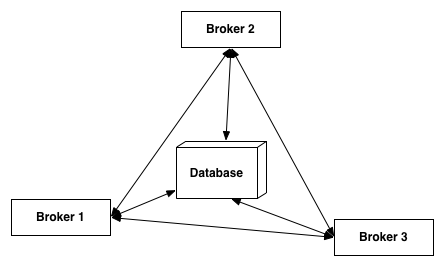
\includegraphics[width=0.65\textwidth]{brokers.png}
\caption{\textit{Visão simplista da arquitectura do servidor.}}
\label{fig:brokers-arq}
\end{figure}

A figura~\ref{fig:brokers-arq} apresenta um esquema simplista das ligações entre os diferentes componentes do servidor. O que se pode retirar do esquema é que os brokers estão ligados entre si e cada um está por sua vez ligado à base de dados.

A base de dados é responsável por armazenar as mensagens persistentes, manter uma sequência que forneça identificadores únicos aos clientes e manter um registo dos endereços dos servidores activos. Todas as restantes acções são da responsabilidade dos brokers. A ligação entre todos os brokers serve dois propósitos:

\begin{enumerate}
\item \textbf{Difundir mensagens}. As mensagens que um broker recebe são difundidas pelos restantes. Isto permite que vários clientes possam subscrever os mesmos canais quando estão ligados a brokers diferentes.
\item \textbf{Informar da actualização na lista de servidores}. Quando existe um novo broker online ou um dos brokers é identificado como inactivo o novo broker ou o broker que identificou o problema, respectivamente, actualizam a base de dados e enviam uma mensagem de actualização a todos os brokers.
\end{enumerate}


\section{Servidor}

É de notar que até este ponto no relatório se faz referência ao servidor como uma componente.
Nesta secção o servidor é analisado como o conjunto das suas componentes, descrevendo-se as funcionalidades de cada componente, meios de comunicação e protocolo.

\subsection{Broker}

Os brokers do servidor são instâncias de uma aplicação desenvolvida em Ruby. Cada instância difere apenas nos endereços de comunicação, o endereço para comunicação com clientes e outro para comunicação com os restantes brokers.
Sendo que cada broker executa num processo Ruby justifica-se que na mesma máquina se executem diversos brokers de forma a tirar partido de paralelismo de processamento (ver secção~\ref{sec:ruby}).
Note-se que cada broker executa numa thread apenas uma vez que foi desenvolvida no paradigam orientado a eventos fazendo uso da ferramenta EventMachine (ver secção~\ref{sec:eventmachine}).

Toda a comunicação no servidor é realizada por websockets, tanto para os clientes como entre os brokers. Mais detalhes no protocol de comunicação na secção~\ref{sec:protocolo}.

\subsubsection{Componentes}
Cada broker executa dois serviços de websockets:

\begin{itemize}
\item um para comunicação com os clientes. Será identificado ao longo do relatório como \textbf{serviço de comunicação}).
\item um para comunicação com os restantes brokers. Será identificado ao longo do relatório como \textbf{serviço de sincronização}).
\end{itemize}

Note-se que ainda que execute dois serviços de websockets que atendem em portas diferentes existe apenas uma thread por broker.

O serviço de comunicação com os clientes é responsável por toda a comunicação com os clientes. Este servidor responde aos seguintes eventos de um cliente:
\begin{enumerate}
\item \textbf{nova ligação}. O serviço é recolhe o próximo identificador único da base de dados e envia ao cliente. Este identificador serve apenas para o cliente poder assinar as suas mensagens ou reconhecer as mensagens de outro cliente (este identificador não tem utilidade ao servidor).
\item \textbf{subscrição de canal}. O serviço procura o canal ou cria um novo e devolve ao cliente uma mensagem de sucesso.
\item \textbf{remoção da subscrição de um canal}. O serviço remove a subscrição do cliente.
\item \textbf{mensagem para diversos canais}. O serviço difunde a mensam pelos respectivos canais e submete para o serviço de sincronização.
\end{enumerate}

\hl{}

\textbf{Novo servidor}
\begin{enumerate}
\item Iniciar o servidor que recebe ligações dos restantes brokers.
\item Registar o endereço do servidor na base de dado
\item Criar a ligação a todos os brokers que estão activos na base de dados.
\item Utilizar cada ligação para informar da actualização da lista de brokers.
\item Iniciar o servidor de websockets.
\end{enumerate}




\section{Protocolo de comunicação}
\label{sec:protocolo}

As mensagens que o servidor reconhecem são no seguinte formato:

[[instructions], message]

Pode resumir-se que é um array que contém uma lista de instruções na posição zero e uma mensagem na posição um. Existem os seguintes tipos de mensagens:

\begin{enumerate}
\item
\texttt{[[``subscribe''], ``channel'']}

Quando a primeira instrução é ``subscribe'' o servidor subscreve o cliente ao canal com o nome que vai no lugar da mensagem.

\item
\texttt{[[``subscribe'', ``persistent''], ``channel'']}

Se o subscribe for acompanhado de um persistent então o canal criado é persistente. Senão subscreve ao canal existente.

\item
\texttt{[[``unsubscribe''], ``channel'']}

Quando a primeira instrução é ``unsubscribe'' o servidor remove a descrição do cliente ao canal com o nome que vai no lugar da mensagem.

\item
\texttt{[[``all''], ``message'']}

Quando a primeira instrução é ``all'' a mensagem é enviada a todos os clientes do servidor (clientes de todos os brokers).

\item
\texttt{[[``channel 1'', ``channel 2''], ``message'']}

Quando a primeira instrução não é ``all'' então todos as instruções são consideradas nomes de canais e a mensagem é distribuída por todos os clientes subscritos ao canal.

\end{enumerate}

\subsection{Ciclo de Vida de um Cliente}

\begin{figure}[H]
\centering
\includegraphics[width=0.65\textwidth]{server_client.png}
\caption{\textit{Ciclo de vida de um cliente.}}
\label{fig:server-client}
\end{figure}

A figura~\ref{fig:server-client} contém um diagrama de sequência que apresenta o básico da interação entre um cliente e o servidor (entenda-se por servidor como um broker do servidor).
Um cliente começa por estabelecer ligação a um dos brokers do servidor. Assim que a ligação é estabelecida o broker devolve um identificador único ao cliente. Esta etapa está identificada no bloco um na figura~\ref{fig:server-client}. Depois esta etapa inicial são três os cenários possíveis servidor

\begin{itemize}
\item
\textbf{O cliente envia uma mensagem}

O cliente envia uma mensagem ao broker (etapa 2 da figura~\ref{fig:server-client}). A mensagem é devolvida ao cliente no processo de broadcast do servidor.

\item
\textbf{O servidor faz broadcast de uma mensagem}

O servidor envia uma mensagem no processo de broadcast de mensagens de outros clientes (etapa 3 da figura~\ref{fig:server-client}).

\item
\textbf{O cliente termina a ligação}

O cliente termina a ligação com o servidor (etapa 4 da figura~\ref{fig:server-client}).
\end{itemize}


\section{Base de Dados}
A base de dados é uma componente centralizada no servidor. É partilhada por todos os brokers e deve encontrar-se num endereço conhecido por todos. Deste modo as características tecnológicas da base de dados relevantes para o projecto são a possibilidade de instalação para \textbf{acesso remoto} e \textbf{controlo de concorrência}.
Nestes termos as opções são variadas, desde MySQL, PostgreSQL, Oracle, Microsoft SQL Server, entre muita outras.

Uma vez que não se pretende tirar grande partido de ferramentas da dimensão do Oracle ou SQL Server é certo que opções com um menor \textit{footprint} são uma melhor opção. Entre MySQL e PostgreSQL não se encontram distinções relevantes no contexto deste problema, mas uma vez que PostgreSQL é a base de dados de preferência da comunidade Ruby será também a adoptada neste projecto como se tinha já referido na secção~\ref{sec:intro-postgres}.

A base de dados é responsável por armazenar as mensagens persistentes, manter uma sequência que forneça identificadores únicos e registar os endereços dos servidores activos.

Funcionalidades da base de dados:
Guardar mensagens dos canais com persistência.
Guardar endereços dos servidores.

na escrita de mensagens nos canais (permite determinar quem enviou primeiro)
na reescrita do estado dos dos servidores
na obtenção de um identificador único para um utilizador

\renewcommand*{\lstlistingname}{SQL}
\lstset{language=SQL, caption={SQL para criar a base de dados}}
\begin{lstlisting}
CREATE SEQUENCE user_id START 1;

CREATE TABLE IF NOT EXISTS sessions (
  id SERIAL PRIMARY KEY,
  name VARCHAR,
  text TEXT);

CREATE TABLE IF NOT EXISTS servers (
  id SERIAL PRIMARY KEY,
  host VARCHAR,
  active BOOLEAN);
\end{lstlisting}

\lstset{language=SQL, caption={SQL para criar a base de dados}}
\begin{lstlisting}
SELECT nextval('user\_id')
\end{lstlisting}


A base de dados é sempre uma necessidade para as mensagens de canais persistentes.
No entanto as restantes funcionalidades podiam ser substituídas.

Para a questão de adequirir um identificador único no sistema para cada cliente a solução podia passar por:
um cliente envia um pedido a todos os brokers para devolver o último identificador, o cliente recolhe todas as mensagens e utiliza o valor mais alto para gerar o próximo identificador. Esta solução teria o problema da concurrência e como tal seria necessária passar um \textit{mutex}, por exemplo, para garantir que apenas um broker pode pedir um identificador de cada vez.

Para identificar os brokers activos podia existir um monitor responsável por fornecer os endereços dos brokers activos a um novo broker e do mesmo modo identificar falhas e informar os brokers.

\section{Testes}

De modo a validar os resultados apresentados pela solução faz-se uma análise comparativa com outras soluções no mercado. Como tal uma instalação do \textbf{RabbitMQ} com o plugin \textbf{RabbitMQ-Web-Stomp} será o contra exemplo para os testes realizados. É de notar que o que este plugin faz é expor o protocolo STOMP (Streaming Text Oriented Message Protocol) através de websockets. A solução proposta pelo ZeroMQ passa pelo mesmo mecanismo como tal não existe qualquer vantagem de escolha.

RabbitMQ é um MOM open source que implementa o protocolo Advanced Message Queuing Protocol (AMQP). Com recurso 

RabbitMQ is open source message broker software (i.e., message-oriented middleware) 
that implements the Advanced Message Queuing Protocol (AMQP) standard.


\section{Conclusion}

Ficou também por se realizar a comparação entre o desempenho entre a aplicação e alternativas ``mainstream'' como RabbitMQ ou ZeroMQ. No entanto note-se que essa comparação não seria de carácter muito justo uma vez que se compara uma aplicação protótio com soluções líders, mesmo não equacionando a heterogenidade de tecnologias.

\section{Glossário}
\begin{description}
\item[canal] Também como conhecido \textit{queue} em outros MOM. É um filtro ao qual um cliente pode subscrever para receber as mensagens para aí enviadas.

\end{description}


\section{Siglas}
\begin{description}
\item[MOM] Vem do inglês \textit{Message-oriented middleware}.
\end{description}

%---------------------------------------------------------------------------------------
%	BIBLIOGRAPHY
%---------------------------------------------------------------------------------------

%\bibliographystyle{plain}
\begingroup
\raggedright
\bibliography{bibliography.bib}
\endgroup

%---------------------------------------------------------------------------------------

\end{document}
